\documentclass{standalone}
\usepackage{tikz}
\begin{document}
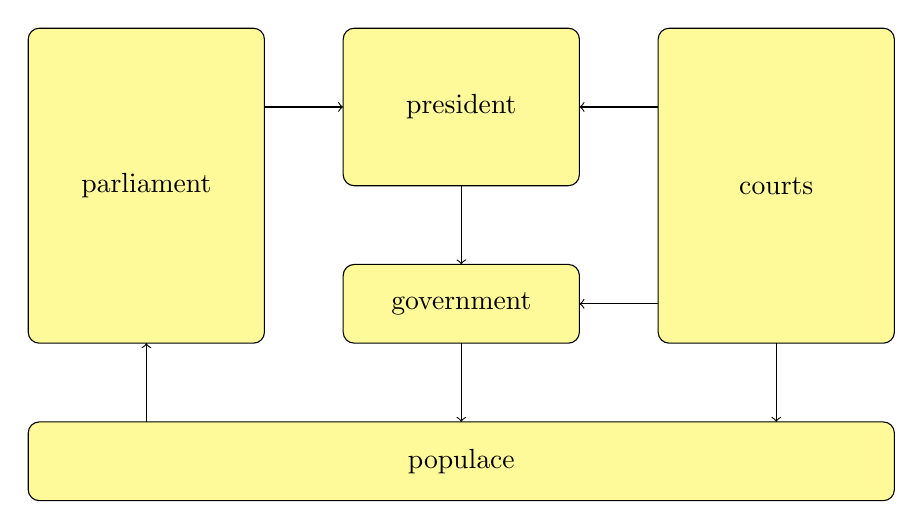
\begin{tikzpicture}
    \tikzset{mybox/.style={fill=yellow!40,rounded corners}}
    \draw[mybox] (-5,0) rectangle node {populace} (6,1);
    \draw[mybox] (-5,2) rectangle node {parliament} (-2,6);
    \draw[mybox] (-1,4) rectangle node {president} (2,6);
    \draw[mybox] (-1,2) rectangle node {government} (2,3);
    \draw[mybox] (3,2) rectangle node {courts} (6,6);
    \draw[->] (-3.5,1) -- (-3.5,2);
    \draw[->] (-2,5) -- (-1,5);
    \draw[->] (0.5,4) -- (0.5,3);
    \draw[->] (0.5,2) -- (0.5,1);
    \draw[->] (3,5) -- (2,5);
    \draw[->] (3,2.5) -- (2,2.5);
    \draw[->] (4.5,2) -- (4.5,1);
\end{tikzpicture}
\end{document}